\section{Estado del arte}
\label{sec:StateOfTheArt}
El desarrollo de esta sección se enfoca en dos temas relacionados al
presente trabajo: la comunicación dominio-vista y el manejo de transacciones
dentro de las interfaces de usuario.

\subsection{Estrategias para la comunicación dominio-vista}
La interfaz de usuario necesita obtener información del dominio para presentar
al usuario, así como actualizar esa información a partir de las acciones del usuario.
La necesidad de intercambiar información entre dominio e interfaz de usuario
entra en conflicto con el objetivo de minimizar el conocimiento entre ambas,
como propone el patrón MVC.

Para solucionar esta contradicción la teoría MVC propone que la
comunicación entre dominio y vista se realice a través de eventos. 
Como se explicó en la Sección \ref{sec:Eventos}, los eventos
permiten formas de comunicación con un muy bajo acoplamiento. 
Sin embargo, son pocos los lenguajes que incorporan un manejo automático de
eventos, por eso se requiere utilizar herramientas tecnológicas adicionales.
A continuación detallaremos las estrategias más utilizadas para atacar este problema.

\subsubsection{\emph{Binding} con eventos manuales}
	En algunas tecnologías que no tienen manejo automático de eventos se obliga a
	los objetos de dominio a disparar eventos \emph{explícitamente} cada vez cambia
	el valor de una de sus propiedades.
	
	Esta técnica es utilizada en
	frameworks como \emph{JFace-DataBinding}\footnote{JFace-DataBinding es un
	Framework de presentación basado en el lenguaje Java y utilizado para la
	construcción del conocido entorno de trabajo \emph{Eclipse}} y el Arena
	actual, que se basan en el estandar de
	\emph{JavaBean}s \cite{sousa00formal}.
	La figura \ref{javabeans} describe el esquema de eventos utilizado en estas
	tecnologías. El framework lleva un registro de los \emph{listeners}
	interesados en cada propiedad de cada objeto, pero se obliga a cada objeto de dominio a:
	\begin{itemize}
	  \item tener una referencia a una instancia de la clase
	  \code{PropertyChangeSupport}
	  \item realizar una notificación cada vez que cambia una de sus propiedades
	  \emph{observables}
	\end{itemize} 

	
	 \begin{figure}[h]
		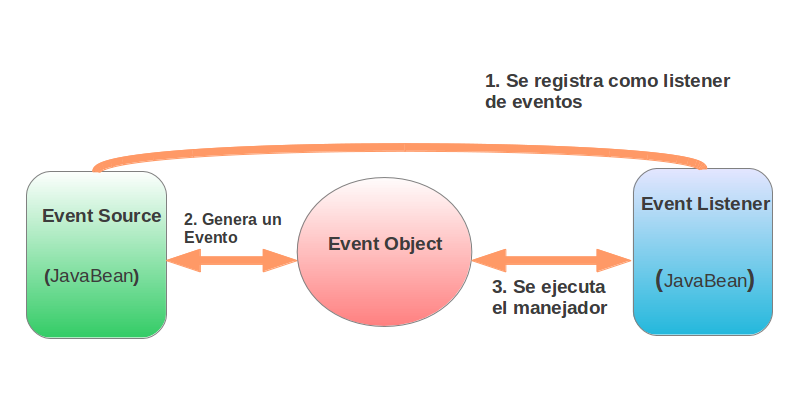
\includegraphics[width=350px, height=200px]{img/javabeans}
		\caption{Esquema de eventos definido por el estándar de \emph{Javabeans}}
		\label{javabeans}
	\end{figure}

	La principal ventaja de esta estrategia es que
	permite una comunicación fluida y desacoplada entre la vista y el modelo.
	El problema es que, al disparar los eventos manualmente se ensucian las clases
	del dominio. Además, obliga a escribir mucho código repetitivo, que hace que
	sea muy fácil cometer errores.

\subsubsection{Formularios web}
	En los formularios web, el binding se realiza atreves del \emph{submit} de un
	formulario; como por ejemplo Wicket\footnote{Wicket es un Framework web MVC
	para el lenguaje Java.}. 
	Se pueden diferenciar dos tipos de submit, submit con refresh y submit con
	ajax.
	 
	\begin {enumerate}
	
		\item{\bf Submit con Refresh}  No se necesita que el dominio dispare eventos
		para realizar el binding, sino que en el momento de renderizar la página se
		leen nuevamente todas las propiedades del dominio.
		Como wicket corre sobre una plataforma web, en el form en cada submit envía  
		toda la pagina, y al volver, la renderiza nuevamente.
		
		Por otro lado, tampoco es necesario tener eventos desde la vista hacia el
		modelo. El concepto de Form decide qué datos son los que hay que volcar de un
		lado a otro.
	
		\item {\bf Submit con Ajax} 
		Es una derivación del anterior, a diferencia de que solo se envía
		una porción de la página, entonces hay que decirle explícitamente que parte
		de la pagina queremos refrescar, para que solo renderice esa parte.

	\end {enumerate}
		
		

%\comment{investigar que hace morphic, preguntar a Guille.
%	Y tal vez otros frameworks\ldots acá preguntémosle a Javi otros modelos de
%	binding.}


\subsection{Manejo de transacciones en la UI}

	En esta sección analizaremos las propiedades ACID, tal como se
	explicó en la sección \ref{sec:ACID},  pero en el entorno de las interfaces
	de usuario.
	Explicaremos las estrategias mas utilizadas en las UIs, y que propiedades ACID
	se cumplen.


	\subsubsection{Interfaces de Usuario sin estado}
		Esta estrategia es muy común en aplicaciones web. Se evita almacenar estados
		en las UIs y se lo delega todo a la base de datos (BD), o bien debe enviarse
		en cada interacción con el cliente.
		
		De esta manera, la	ausencia de datos fuera de la BD, garantiza que no se
		rompen estas propiedades.
		
		Una de las desventajas que tiene este sistema es que si se esta en el
		paradigma de la programación orientada a objetos, en cada pedido de datos
		se tiene que reconstruir todo el grafo de objetos, y si el grafo es muy grande,
		esta operación se vuelve repetitiva y lenta.
		
%		\comment{Otos sistemas que utilizan dicha estrategia son las
		% \emph{Arquitecturas orientada a Servicios} y la \emph{Unidad de Trabajo}}
		
	\subsubsection{???}
		\comment{En este esquema se almacenar la información durante la edición, en
		algún lugar fuera del objeto. Como consecuencia se postergan las validaciones de negocio hasta la
		finalización de la edición , o se duplica la validación de negocio en la uis.}
	
	
	\subsubsection{Clonar al editar}
	
		Clonar al editar es una estrategia que se basa en la idea de no modificar el
		objeto, hasta que se confirme la edición. Cuyo funcionamiento se basa en 
		clonar el objeto, y modificar el objeto clonado. Cuando se confirma la
		edición, se impacta los cambios del clon en el objeto original.
		
		Con dicha estrategia la Atomicidad se cumple, ya que solo se pasan los datos
		al original, solo cuando se confirma la operación.
		En caso de que se quiera cancelar la operación, solo se tiene que tirar la
		copia.
		
		Con el Aislamiento hay problemas si varios usuarios intentan modificar un
		objeto, cada uno tendría una copia, pero si mas de uno confirman sus cambios,
		los datos quedarían inconsistentes.
		
		La desventaja que tiene esta estrategia es que se pierde la identidad del
		objeto, copiar todos los datos de un objeto a otro, hay que hacerlo a mano, y
		esta operación hay que hacerla dos veces, tanto para hacer la copia, y para
		confirmar los cambios.
